% http://tex.stackexchange.com/questions/17579/how-can-i-design-a-book-cover

\documentclass{book}
\usepackage{graphicx}

\usepackage{hyperref}
\usepackage{float}
\usepackage[margin=0.5in]{geometry}
\usepackage{caption}

%\usepackage{fancyvrb}
\begin{document}
\clearpage
%% temporary titles
% command to provide stretchy vertical space in proportion
\newcommand\nbvspace[1][3]{\vspace*{\stretch{#1}}}
% allow some slack to avoid under/overfull boxes
\newcommand\nbstretchyspace{\spaceskip0.5em plus 0.25em minus 0.25em}
% To improve spacing on titlepages
\newcommand{\nbtitlestretch}{\spaceskip0.6em}
\pagestyle{empty}
\begin{center}
\bfseries
\nbvspace[1]
\Huge
{\nbtitlestretch\huge
TA Manual for the Controls Lab}

\nbvspace[1]
\normalsize

% TO WHICH IS ADDED MANY USEFUL ONE\    LINERS AND CODE SO THAT\    YOU CAN AWK LIKE A HAWK
\nbvspace[1]
\small BY\    \Large Justin Pearson\\[0.5em]
\footnotesize Humble graduate student \\ January 2017
% AUTHOR OF ``A WORKING ALGEBRA,'' ``WIRELESS TELEGRAPHY,\    ITS HISTORY, THEORY AND PRACTICE,'' ETC., ETC.

\nbvspace[2]


% \begin{figure}
%   \centering
%     \reflectbox{%
%       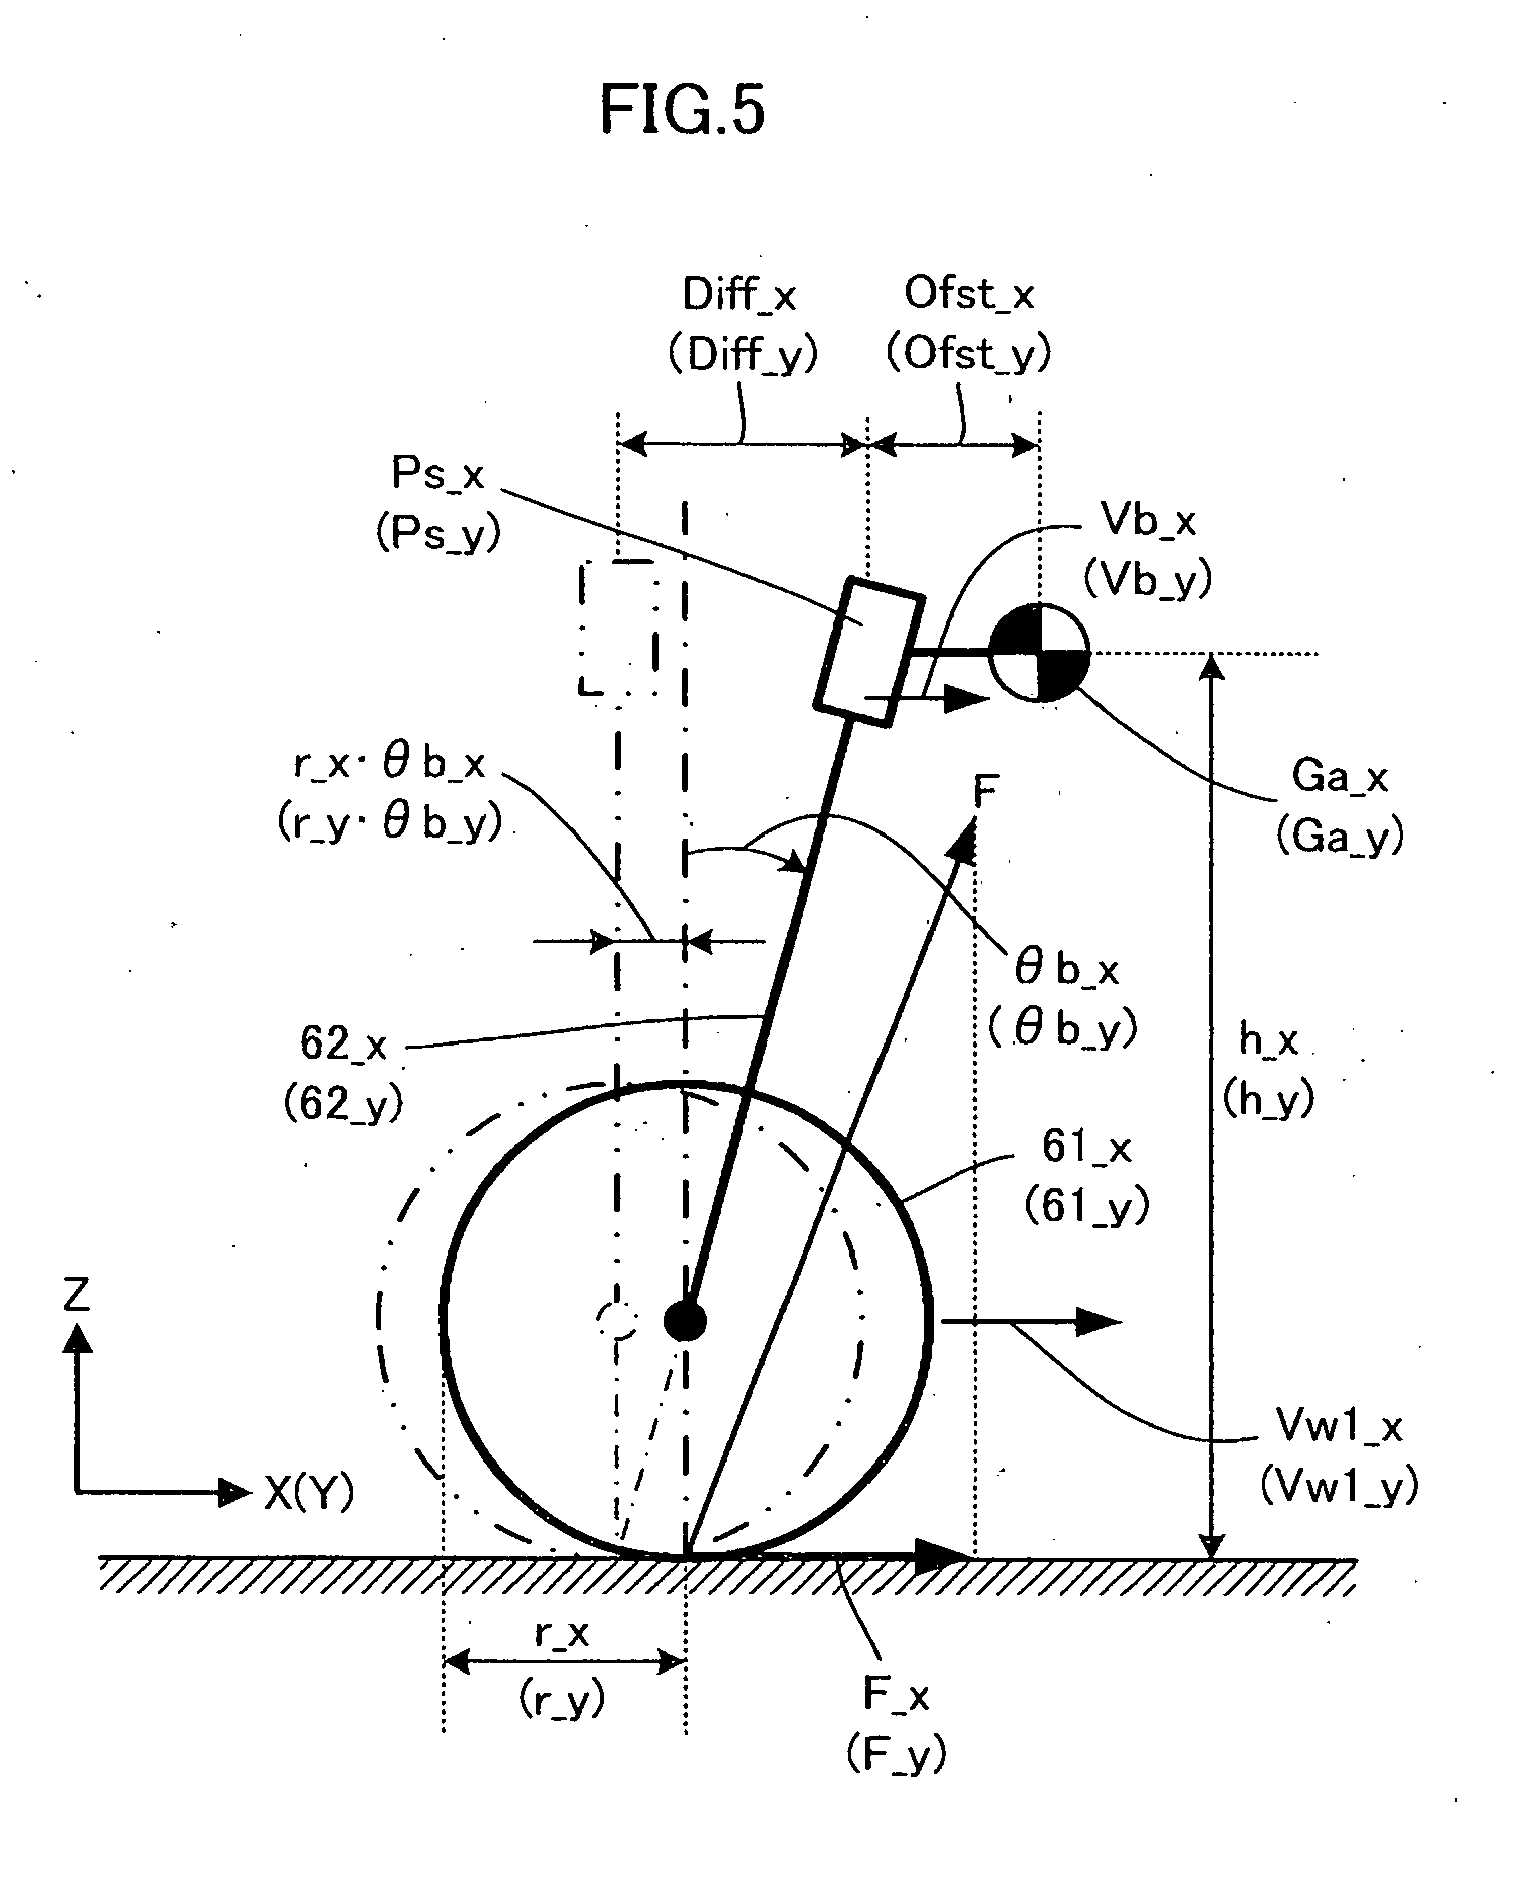
\includegraphics[width=0.5\textwidth]{./Images/imgf0005.png}}
%   \caption{A picture of the same gull
%            looking the other way!}
% \end{figure}

\begin{figure}[H]
\centering
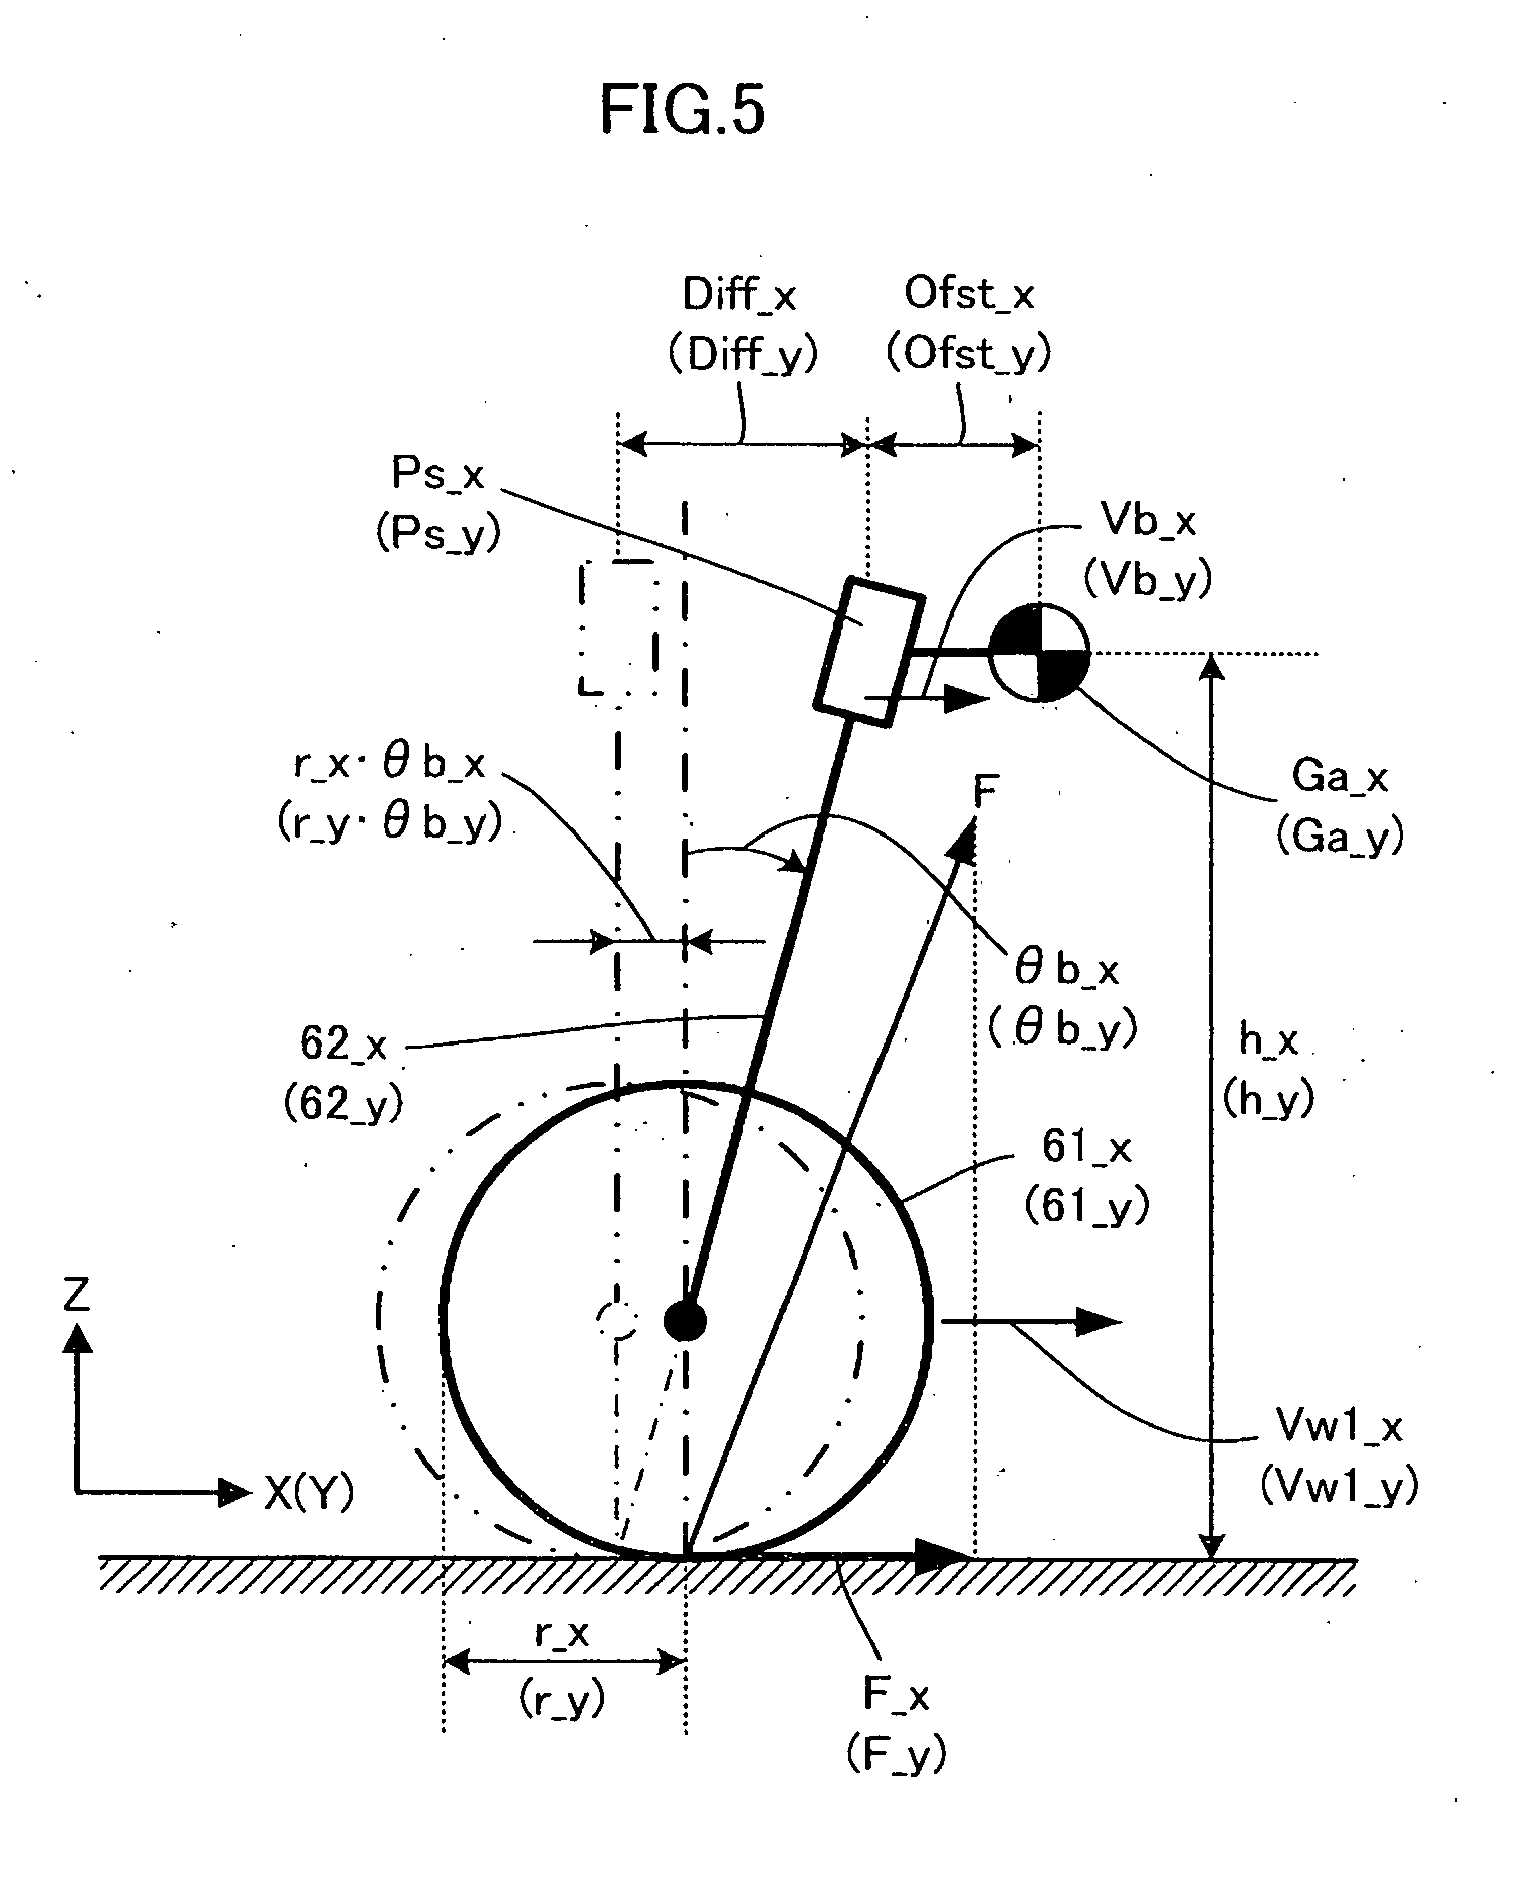
\includegraphics[width=.5\textwidth]{./Images/imgf0005.png}
%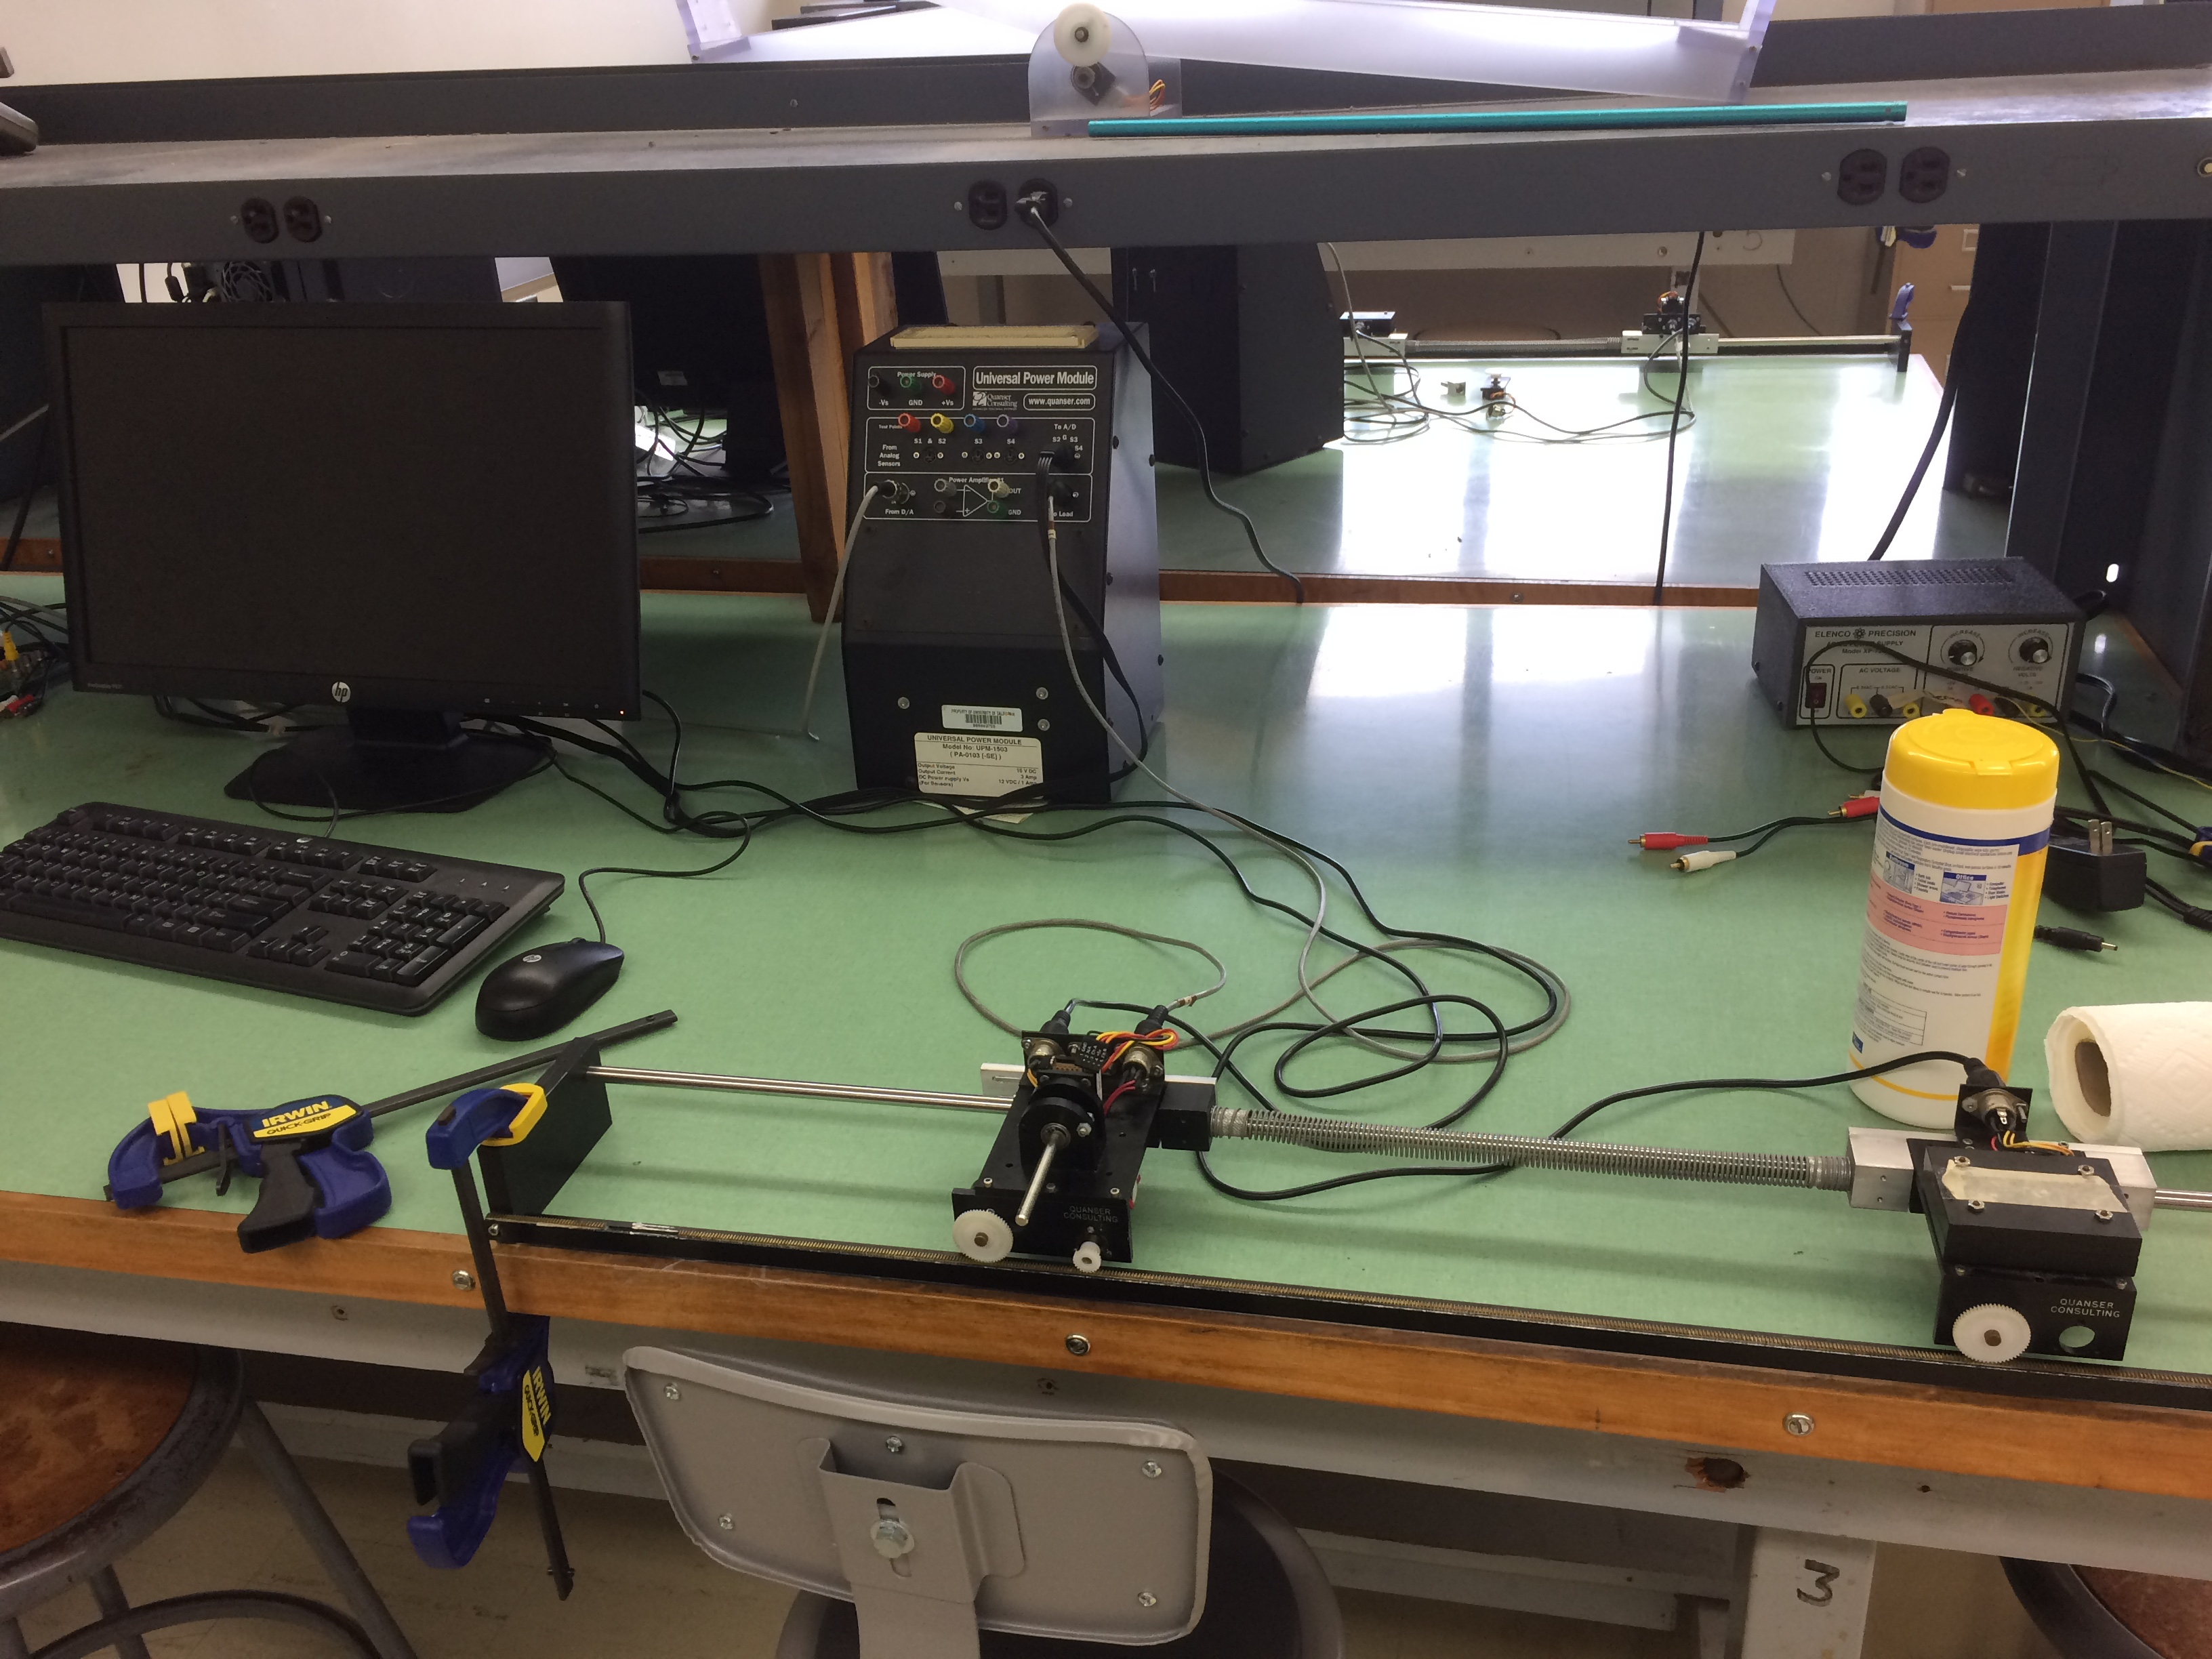
\includegraphics[width=5in]{./Images/IMG_6727.JPG}
  \caption{Inverted pendulum type vehicle. \\ United States Patent 8,744,688}
\end{figure}
\nbvspace[3]
\normalsize

This document lives at 

\url{https://github.com/justinpearson/UCSB-Quanser-Inverted-Pendulum-Lab-Manual}

% DOHA\    \large
% PUBLISHED IN THE WILD
\nbvspace[1]
\end{center}
\end{document}